\section{Dataset Visualization} \label{sec:res_dataset}

\subsection{Label groups}

Figures \ref{fig:res/statelevel_pbr} and \ref{fig:res/statelevel_xy} were created from the final dataset as processed according to section \ref{sec:impl/dataset}. However, instead of using the data as input for classification, it is segmented into the level and state label groups and plotted over time-on-trial. As such, each of the green-, blue-, red- and magenta-colored graphs in these figures represent average values over 43 trials. The same number of trials were used to generate the blue-colored histogram above each plot. Each bar in the histogram represents one 50ms interval. Their heights are normalized according to the number of blinks during each interval.

As is evident from their titles, each row of plots represents one difficulty level of the N-Back task. Additionally, all are marked with black vertical lines along the time axis. These are meant to indicate the points in time where the task transitions from one state to another, as described in section \ref{sec:impl/dataset}. The respective state at each time instance is indicated by the "idle," "onset," "execution," and "offset" labels at the top of each plot.

\begin{figure}[h]
    \centering
    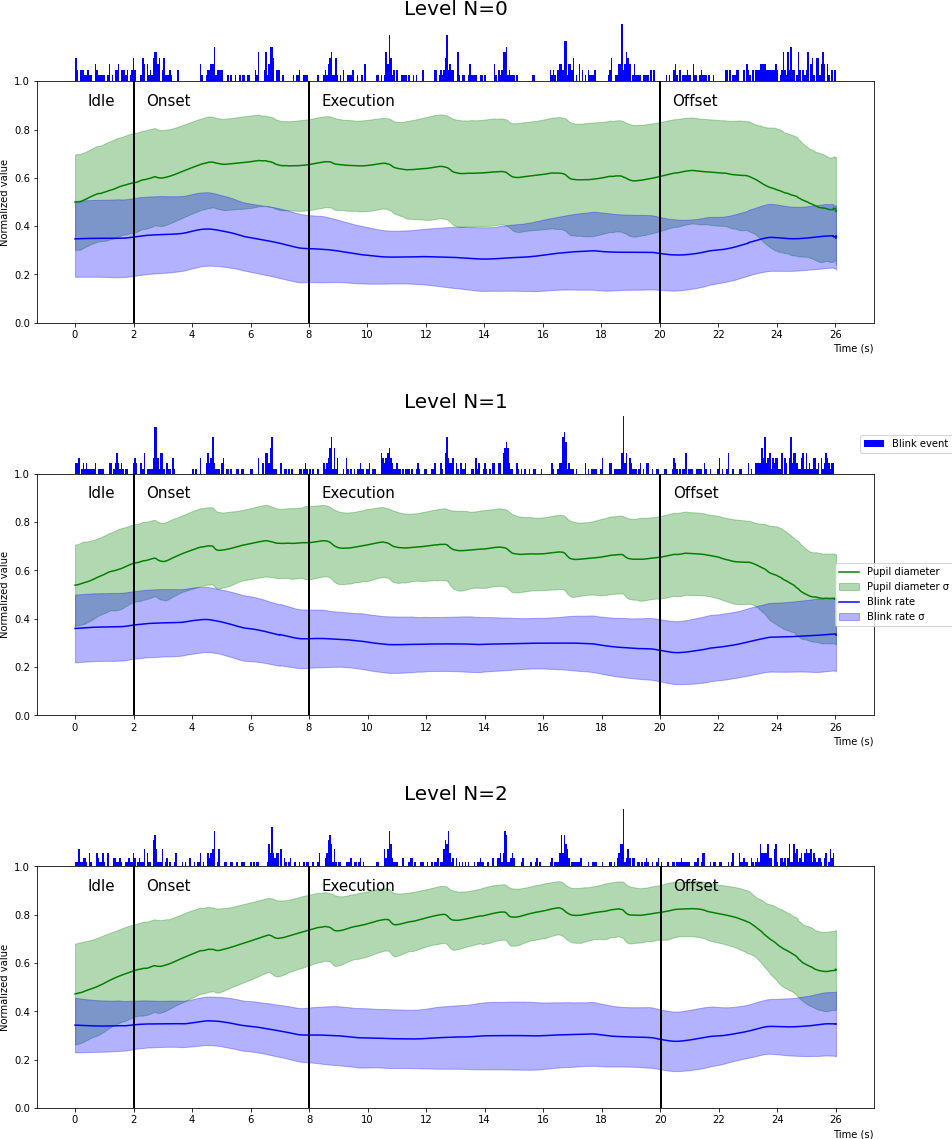
\includegraphics[width=\textwidth]{figures/impl_statelevelvisualization_pbr.png}
    \caption{Visualization of state and level labels of the processed dataset. The green and blue graphs represent the pupillary diameter and blink rate data channels, respectively. The blue histogram represents individual blink occurrences during 50ms intervals throughout the trial. Black vertical lines indicate task state transitions.}
    \label{fig:res/statelevel_pbr}
\end{figure}

\begin{figure}[h]
    \centering
    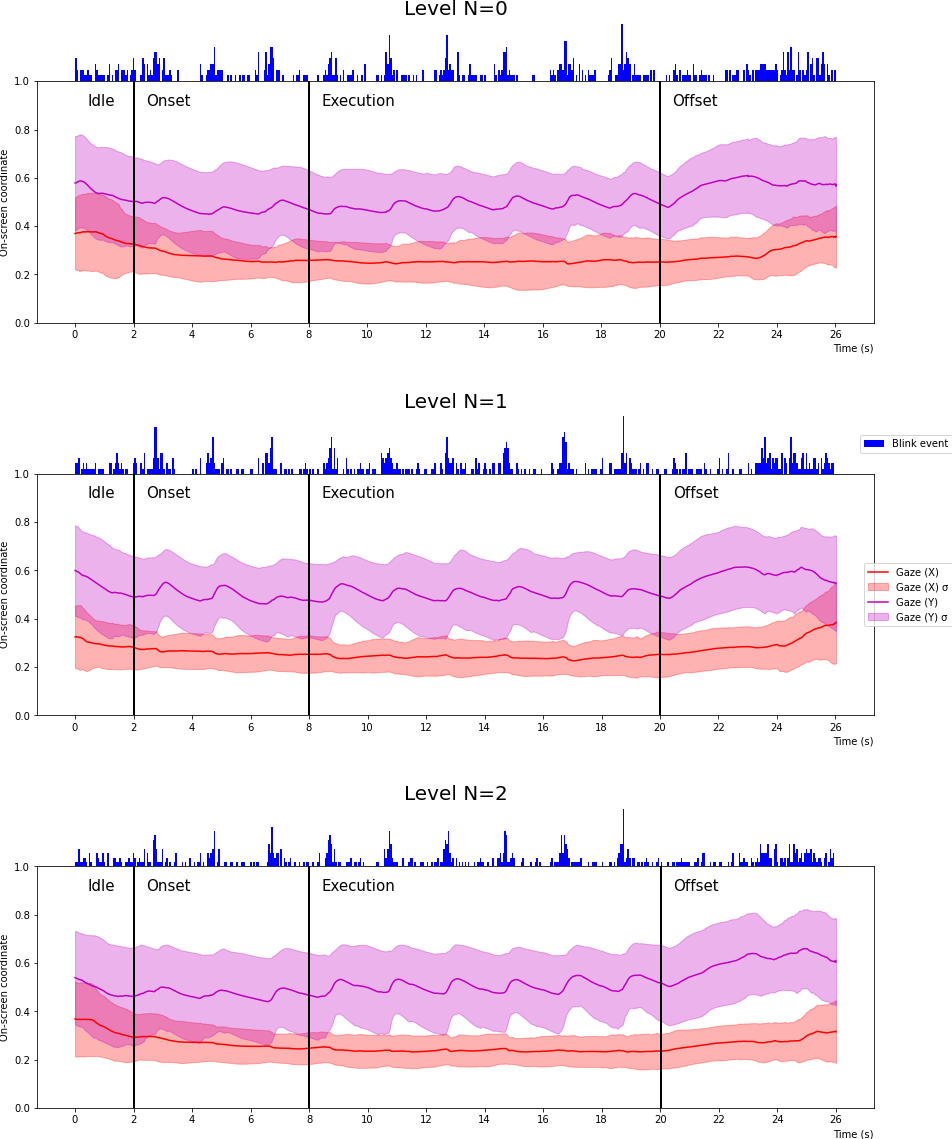
\includegraphics[width=\textwidth]{figures/impl_statelevelvisualization_xy.png}
    \caption{Visualization of state and level labels of the processed dataset. The magenta and red graphs represent the on-screen x- and y-coordinate data channels, respectively. The blue histogram and black vertical lines are similar to figure \ref{fig:res/statelevel_pbr}.}
    \label{fig:res/statelevel_xy}
\end{figure}

\subsection{Task Exposure}

Figure \ref{fig:res/taskexposure} was generated similarly to figures \ref{fig:res/statelevel_pbr} and \ref{fig:res/statelevel_xy}. However, this figure demonstrates how continuous task exposure affects the data. Plot rows each represent one data channel, as is evident from their titles. In each plot, graphs are colored by which time during task exposure they were recorded. For instance, the green graph comes exclusively from the first quarter of the recording session (first 15 minutes). The blue comes from the second quarter (15-30 minutes), and so on. These plots are also indicated with vertical lines representing task states, similar to the above figures.

\begin{figure}[h]
    \centering
    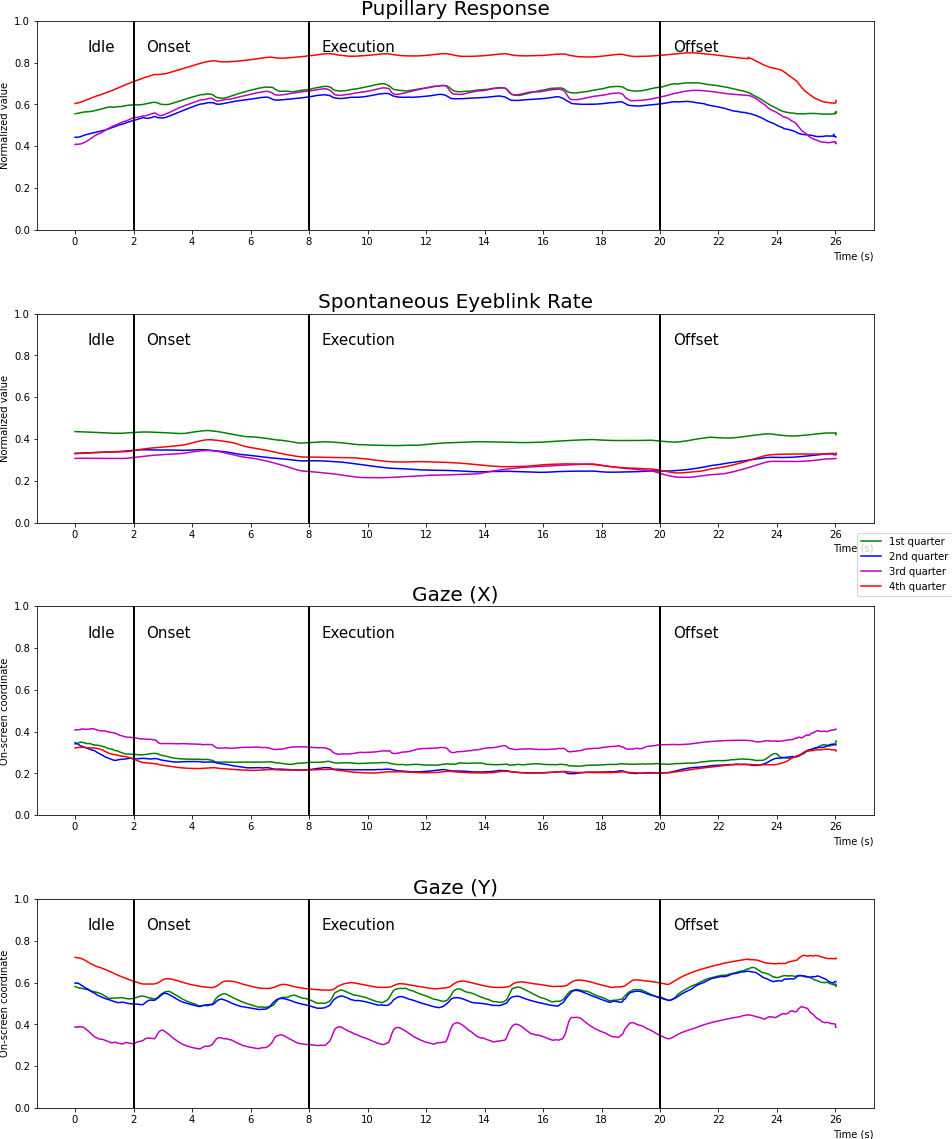
\includegraphics[width=\textwidth]{figures/impl_taskexposurevisualization.png}
    \caption{Visualization of task exposure effect in dataset. Graphs are color-coded by which quarter of task exposure they were recorded. The black vertical lines are similar to figure \ref{fig:res/statelevel_pbr}}
    \label{fig:res/taskexposure}
\end{figure}
\FloatBarrier